In this chapter we turn to the implementation of the function $G_T$ by discussing a method to learn the function $\Gamma$. We apply our methodology to some chaotic attractors. Most notably, we consider the reconstruction of the chaotic attractor of the double pendulum - an  attractor that has not been successfully reconstructed because of its intricate structure. In fact the previous data-driven approaches also have not been successful in building a model from the double pendulum. 



%We then indicate where this implementation differs from previous work done by (\cite{manjunath2021universal}) and empirically show that the SDD of $G_T$ are less functionally complex than $\Phi_{k, \theta}$ or $T$ by considering the Pearson correlation coefficient. Finally, we present and discuss some numerical results for a focus system of this project: the double pendulum. We also consider other chaotic attractors.

\section{Implementing $G_T$}
The map $G_T$ is implemented by applying the functions $\Gamma$, $g$ and the projection function $\pi_2$ in the relevant order as described by the equations~\ref{eqns_from_data}. To reach this point, one must first learn $\Gamma$.
After first normalising the data to ensure that it has zero mean value and lies within the range $[-1,1]$ and required zero-padding(see paragraph below for further discussion), we continue by driving the system with external input through the function $g$.

From \eqref{eqn_driving} we know that $g(u,x) = (1-a) x + a \tanh(Au + \alpha B x)$. Recall that $g$ is SI-invertible. We refer to $A$ as the input matrix and $B$ the reservoir matrix. 

We make use of a Recurrent Neural Network (RNN) in our implementation to project the data on to a higher dimensional space, but we do not train the RNN in the conventional manner. \ednote{B: Should we say what the conventional manner is?} A few words about the RNNs: RNNs are widely used in the literature for temporal processing of data as a type of deep learning technique. They take the form of equations considered to be discrete-time version of continuous dynamical systems modelling a neural network of neurons \cite{jaeger2001echo}.

We implement a feedforward network, (a network with no memory, unlike the RNN)\ednote{B: Expanded sentence s.t. FFN is in more context} required to learn $\Gamma$ in the \emph{Python} programming language and making use of the \emph{Scipy} library, alongside the \emph{Keras} package in the \emph{Tensorflow} library \ednote{B: Is this something you want me to write in? M: We do not implement the RNN, but the FN that learns Gamma through the Tensorflow. We called the RNN + FN set up a RCN in Adriaan's paper. FYI: FN's work only if there is a definite relationship between the $u_n$ and $u_{n+1}$ which is rare in temporal data.
RNNs with ESP work when there is a definite relationship between $(\ldots,u_{n-1},u_n)$ and $u_{n+1}$ and is suited for temporal processing.}.

If the RNN we will be using in the next step has $N$ neurons, then $A$ and $B$ are each $N\times{N}$ matrices. Inputs $u_n$ of dimension $K < N$ are padded by zeroes (as remarked earlier) to embed the input in a space of dimension $N$. As we do not need the entire left-infinite history of input, an arbitrary initialisation of the system with initial values followed by the driving of the system with the function $g$ means that the generated values will approach the actual solution elements in a uniform manner thanks to the UAP that we had discussed in the preceding chapter.

Thirdly we prepare the network. Utilising a network $N$ neurons (the same value $N$ as in the dimensions of the matrices $A,B$). Learning of $\Gamma$ is done using the Adam Optimiser where the means square error (MSE) loss function is optimised. The system is trained several times (in our case 4) with incrementally smaller learning rates on each run (0.001 and thereafter divided by 10 at each run). 
Additional parameters such as the number of network-layers, neurons per layer and training-length are presented case-by-case below.

We then reach the prediction step. Making use of $g$'s SI-invertibility and $g$ as defined in \eqref{eqn_driving}, we have the following expression for $u_n$ replicated from~\eqref{eqn_SI_RNN}.
\begin{equation*}
  u_n := A^{-1}\bigg(\overline{\tanh}^{^{-1}}\frac{1}{a}\Big(x_{n+1}-(1-a)x_n\Big) \bigg) - \alpha B x_n
\end{equation*}
    
The two model equations for learning from data~\eqref{eqns_from_data} allows us to determine what the state $x_{n+1}$ at time $n+1$ will be. 
We specifically remind ourselves of \[x_{k+1}=\pi_2 \circ (\Gamma, \pi_2) \circ (\pi_2,g) (u_k,x_k)\]

\section{Delay Coordinates}

We also consider a more general problem of learning an attractor of dynamical system when only observations of an orbit are given. Explicitly, if $(W,T)$ is a dynamical system with dynamics generated by $w_{n+1}=Tw_n$, and if $\theta:W \to \mathbb{R}$ is an observable, then the task is to learn a dynamical system that is topologically conjugate to $(W,T)$ and predict $\theta(w_{m+1}),\theta(w_{m+2}),...$ using the data $\theta(w_{0}),\theta(w_{1}),\ldots,\theta(w_{m})$.  So how do we do it?
Suppose the input generated from the delay-coordinate map $\Phi_{\theta,2d}(\theta(w_{n})) := (\theta(w_{n-2d}),\ldots,\theta(w_{n-1}),\theta(w_{n}))$ is such that Takens delay embedding theorem (see Theorem~\ref{Thm_Takens}) holds, in which case, there exists a homeomorphism  $F_\theta: \Phi_{\theta,2d}(\theta(w_{n})) \mapsto \Phi_{\theta,2d}(\theta(w_{n+1}))$. Then if we feed  the input values $u_n := \Phi_{\theta,2d}(\theta(w_{n}))$ to a driven system $g$ that is SI-invertible and has USP, the induced system $(Y_F,G_F)$ would be topologically conjugate to the inverse-limit space of
$(\Phi_{\theta,2d}(W), F_\theta)$ as in Theorem~\ref{Thm_CET}, and hence one could forecast $u_n,u_{n+1},\ldots$. In other words, one could forecast  the values $\theta(w_n), \theta(w_{n+1}),\ldots$ by feeding these observations as delay coordinates. The advantage of feeding delay-coordinates to a driven system is that the embedding is stable in the sense of global dissipativity that we have described in the previous chapter, i.e., $Y_F$ is made to contained in an attractor of a mapping induced on $Y_F$ that is induced by $g$. 

We note that the twin equations together~\ref{eqns_from_data} generate a model from data. For a chaotic system, a small amount of noise due either to the input-noise or computational error would cause the solutions from two accurate models with the same initial conditions to  diverge as they are not identical. \ednote{B: edited this sentence} However, statistically, they would be the same since due to ergodic theory all typical orbits have the same visiting frequency to any region of the phase space of the dynamical system. \ednote{B: I'll need to recap this sentence with you before presenting as it's new to me.} To illustrate that we plot the densities of the trajectories of the actual and predicted solutions. 

Our implementation of the reservoir(A) and input(B) matrices in the RNN makes use of sparse matrices. We discuss three specifics relating to this concept. Firstly, the matrices are assigned a variable density in terms of the amount of non-zero entries and are scaled to have values within the range $[-1,1]$. For this, we make use of \textit{Python's SciPy} library and specifically the \textit{Sparse, LinAlg} modules. In our experiments, we generally opted for a density ratio of 10\%-25\%.
Secondly, we opted to enforce the requirement that both matrices be well-conditioned, i.e. that they have a condition number of \~1. The condition number of a matrix $M$ (denoted $cond(M)$) is the product of the matrix norms of the matrix $M$ and its inverse $M^{-1}$ and is a measure of the sensitivity of output of a matrix multiplication when an input is changed. \textbf{(Cite.)}\ednote{Ask M: Cite specific resource?} By ensuring a condition number close to 1, we also ensure that our driven function $g$, depending on the matrices $A$ and $B$, will not be sensitive to adjustments in the input. In so doing we then also guarantee another form stability. \ednote{B: Not complete enough. Edit further and cite}

Lastly, we ensure the matrix $B$ has unit spectral radius. This is necessary due to the Causal Embedding Theorem~\ref{Thm_CET} which can then guarantee the existence of semi-conjugacy between the systems $(Y_T, G_T)$ and $(\widehat{U}_T, \widehat{T})$. In fact, the theorem actually requires that $\alpha{B}$ have spectral radius $<1$, so we impose the restriction $\alpha<1$ and consider only the matrix $B$'s spectral radius from thereon.


Note that to learn $\Gamma: (x_{n-1},x_{n}) \mapsto u_n$ through our feedforward network, we could learn the principal components of $(x_{n-1},x_{n})$ as well. 
We employ this since it provides slightly better results empirically but is not essential.

Principal components are used only for a more efficient state representation to possibly reduce learning errors; it is not for a lossy approximation since we use all principal components \textbf{(Cite.)}\ednote{Ask M: Is there a specific resource to cite?}.
More explicitly, denote $X_{1:N}$ as the matrix with the first $N$ states of the network data represented by row vectors. If $X_{1:N}=U\Sigma P^T$\ednote{Expand here} represents the singular value decomposition of $X_{1:N}$ \ednote{Ask: Is there a specific resource to cite?}, we then denote the principal component matrix $P$, and the principal components are given by 
 $Z_{1:N}=X_{1:N}P.$
These principal components are then used to train a feedforward neural network. Denote the row vectors of $Z_{1:N}$ by 
$z_i^T, i=1,2,\cdots,N$ and the neural network by $NN$, the network is subsequently trained to learn an approximation of the map
$NN: (z_{n-1},z_n) \mapsto  u_n.
$
The learnt approximation of $NN$ can be used to approximate $\Gamma$ since 
$$
NN\left( \begin{bmatrix} 
P^Tx_{n-1} \\
P^Tx_n
\end{bmatrix}
\right) = NN \circ 
\begin{bmatrix}
P^T & 0 \\
0 & P^T 
\end{bmatrix}\begin{bmatrix}
x_{n-1}\\
x_n
\end{bmatrix} = u_n = \Gamma(x_{n-1},x_n).
$$


\section{Experimental Results}
In this section we showcase numerical results pertaining to 3 attractors that were simulated using the methodology described. We first consider a simple physical system that exhibits complicated dynamics.
\subsection{Double Pendulum}

The Double Pendulum consists of two pendulums fastened to one another such that the system moves as a whole. The first (or higher pendulum) is attached to a fixed point while the second is attached to the endpoint of the first. (See below)
This system is a classical example of a system exhibiting chaos and is often used as explanation of the very well-known Butterfly Effect. \ednote{B: Originally though a reference here was needed, but no longer think so.} Consider again~\ref{fig:dp_sdic}.
The system has four variables: angle and angular velocity of each pendulum rod. An ideal system is assumed where the rods are massless and no friction in the pivots are considered.
\begin{figure}[ht]
  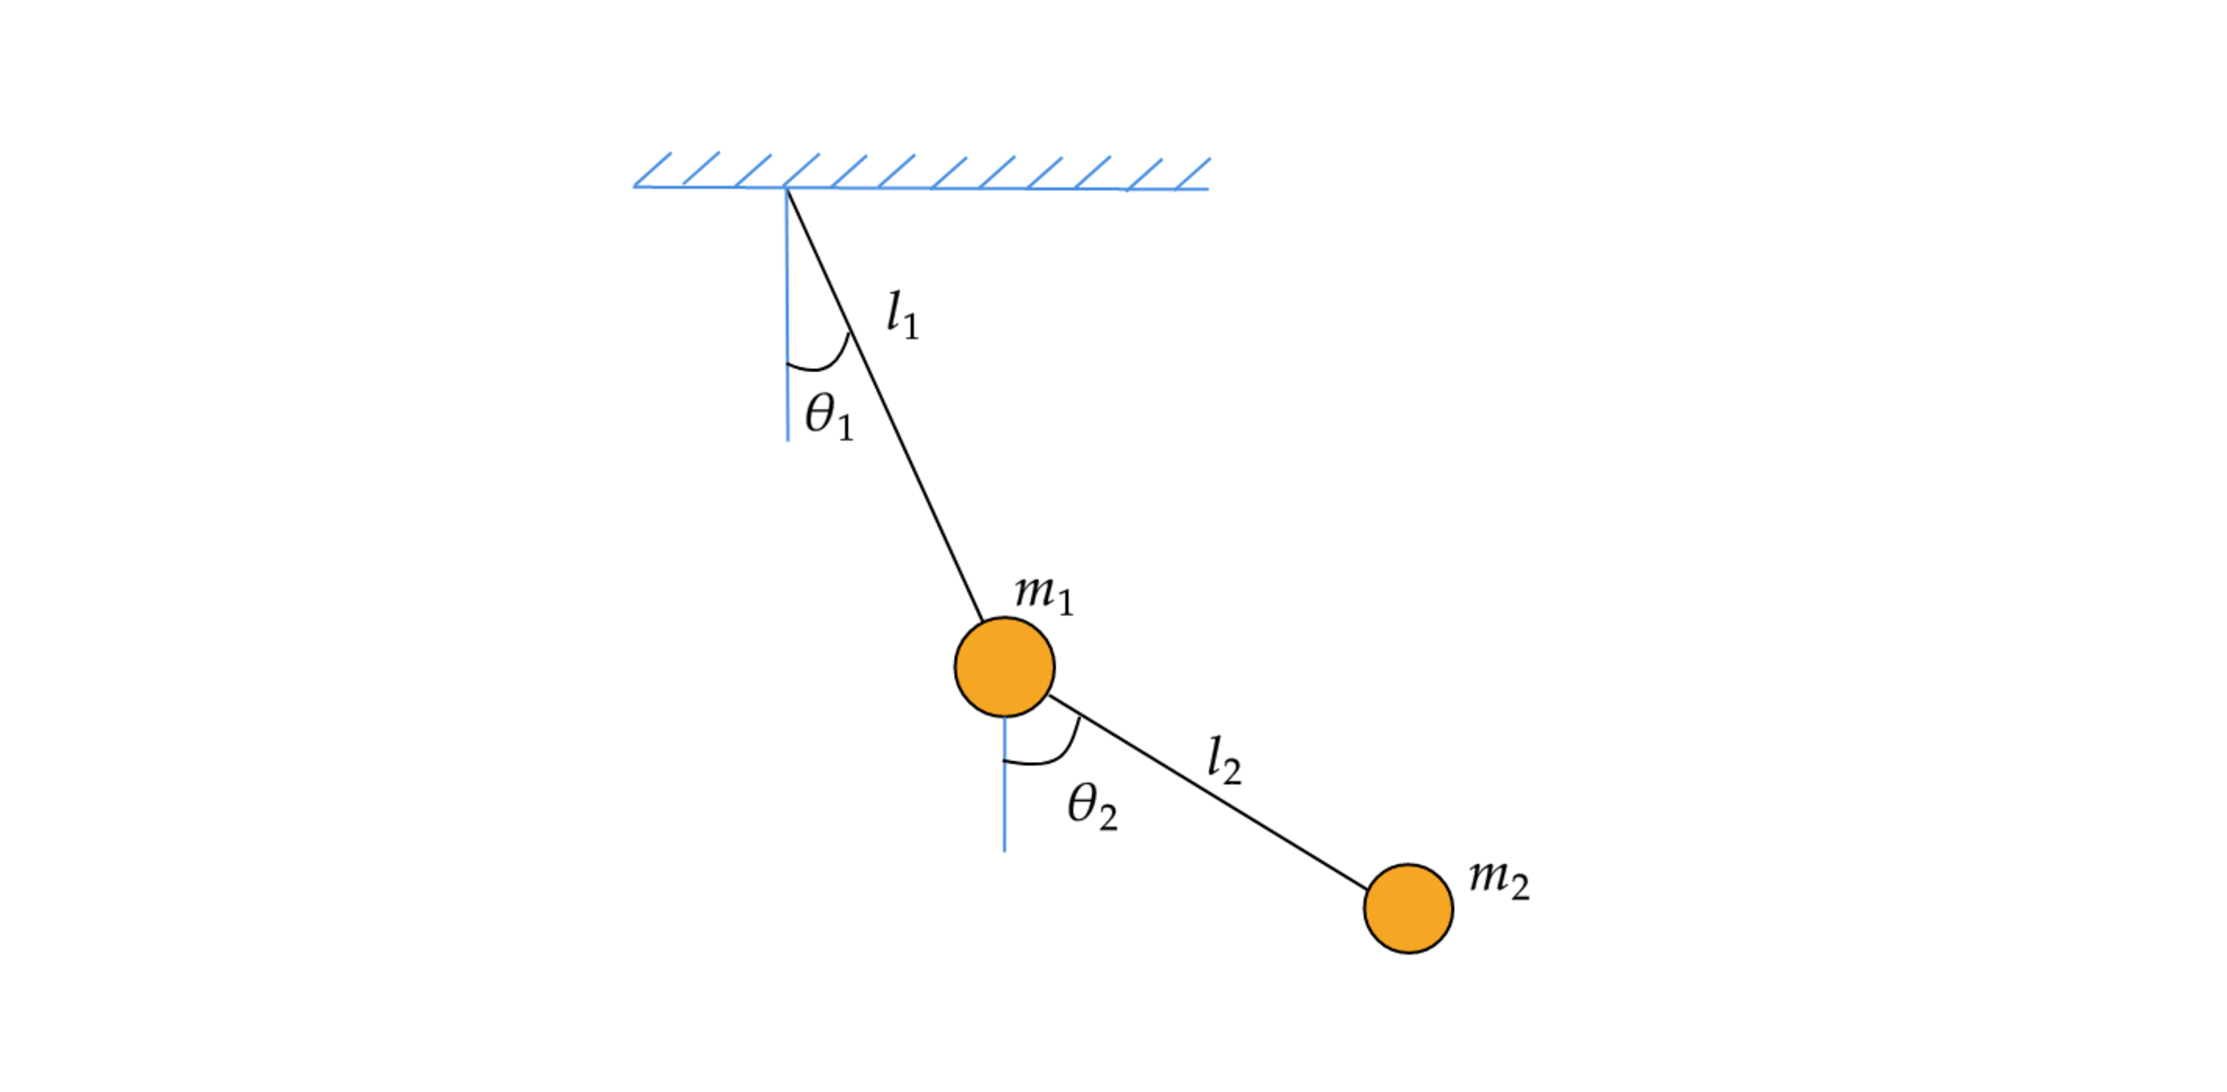
\includegraphics[scale=0.35]{Graphs/_dp_setup.eps}
  \centering
  \captionof{figure}{Pictorial representation of the setup of a DP. Image taken from~\cite{DPSetup}}
  \label{fig:dp_setup}
\end{figure}

The scalar equations of motion are derived using Newtonian physics and are reproduced from~\cite{DPFormulas} in~\ref{eqns_dp}. Each pendulum component has an associated mass of the head, $m$, and length of the rod, $L_i$. Acceleration due to gravity is denoted by $g$ and initial velocities by $\dot{\theta}$
\begin{eqnarray}\label{eqns_dp}
  \ddot{\theta_{1}}  = \frac{-g(2m_1+m_2)\sin{\theta_1} - m_2g\sin(\theta_1-2\theta_2) - 2\sin(\theta_1-\theta_2)m_2({\dot{\theta_{2}}}^{2}L_2 + {\theta_{1}'}L_1\cos(\theta_1-\theta_2))} {L_1(2m_1 + m_2 -m_2\cos(2\theta_1 - 2\theta_2))}
  \\
  \ddot{\theta_{2}} = \frac{2\sin(\theta_1-\theta_2)(\theta_{1}'^{2}L_1(m_1+m_2) + g(m_1+m_2)\cos\theta_1 + \dot{\theta_{2}}^{2}L_2m_2\cos(\theta_1-\theta_2))}{L_2(2m_1 + m_2 -m_2\cos(2\theta_1 - 2\theta_2))}
\end{eqnarray}

The second-order system is converted to a first-order ODE system and solved using the Runge-Kutta numerical method.  
Here we chose the values $m_1=2.0$, $m_2=2.0$, $L_1=1.5$ and $m_2=1.5$ with initial velocities $v_1=1.5, v_2=-2$ for the respective pendulum heads.
Undamped DP data-sets were generated and used in this project due to the requirement that the map $T$ be surjective that we must not forget. 
An example of this would be the case of a DP exhibiting energy-loss (i.e. where the map $T$ is not surjective). In such a case, the attractor is a single point in the phase space when the double pendulum comes to rest. 
It must be mentioned once again that if we use data outside the attractor, learning is not reliable. To see this, consder the graphs ~\ref{fig:damped_pendulum} and ~\ref{fig:dp_notsurjective}.

\begin{figure}[ht]
  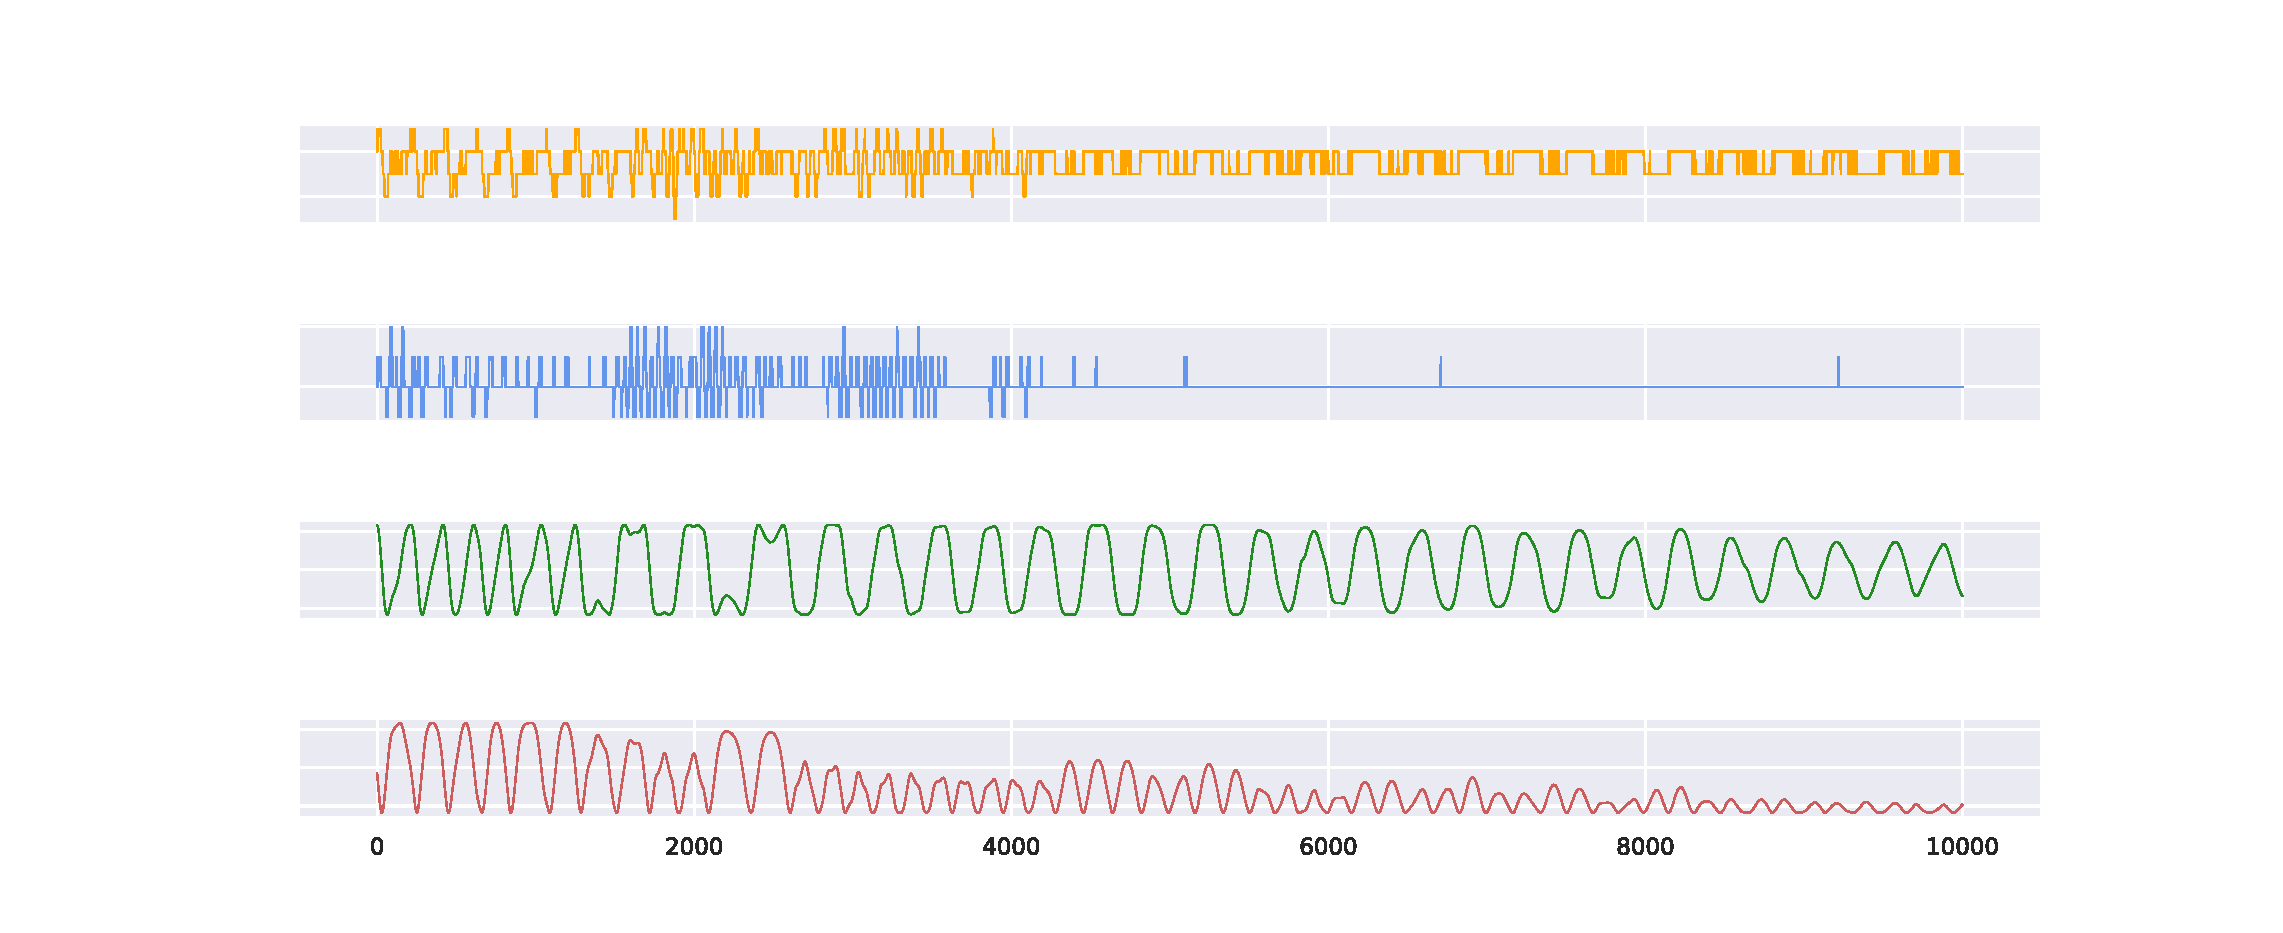
\includegraphics[scale=0.4]{Graphs/_dp_dying.eps}
  \centering
\caption{$x$- and $y$-coordinates of the two pendulum heads plotted for a dataset that exhibits dying oscillations. The map generating the (four-dimensional data) for a damped pendulum is not surjective. Data obtained from chaotic double pendulum dataset generated from videos takes of experimental pendulums~\cite{asseman2018learning}}
\label{fig:damped_pendulum}
\end{figure}



\begin{figure}[ht]
  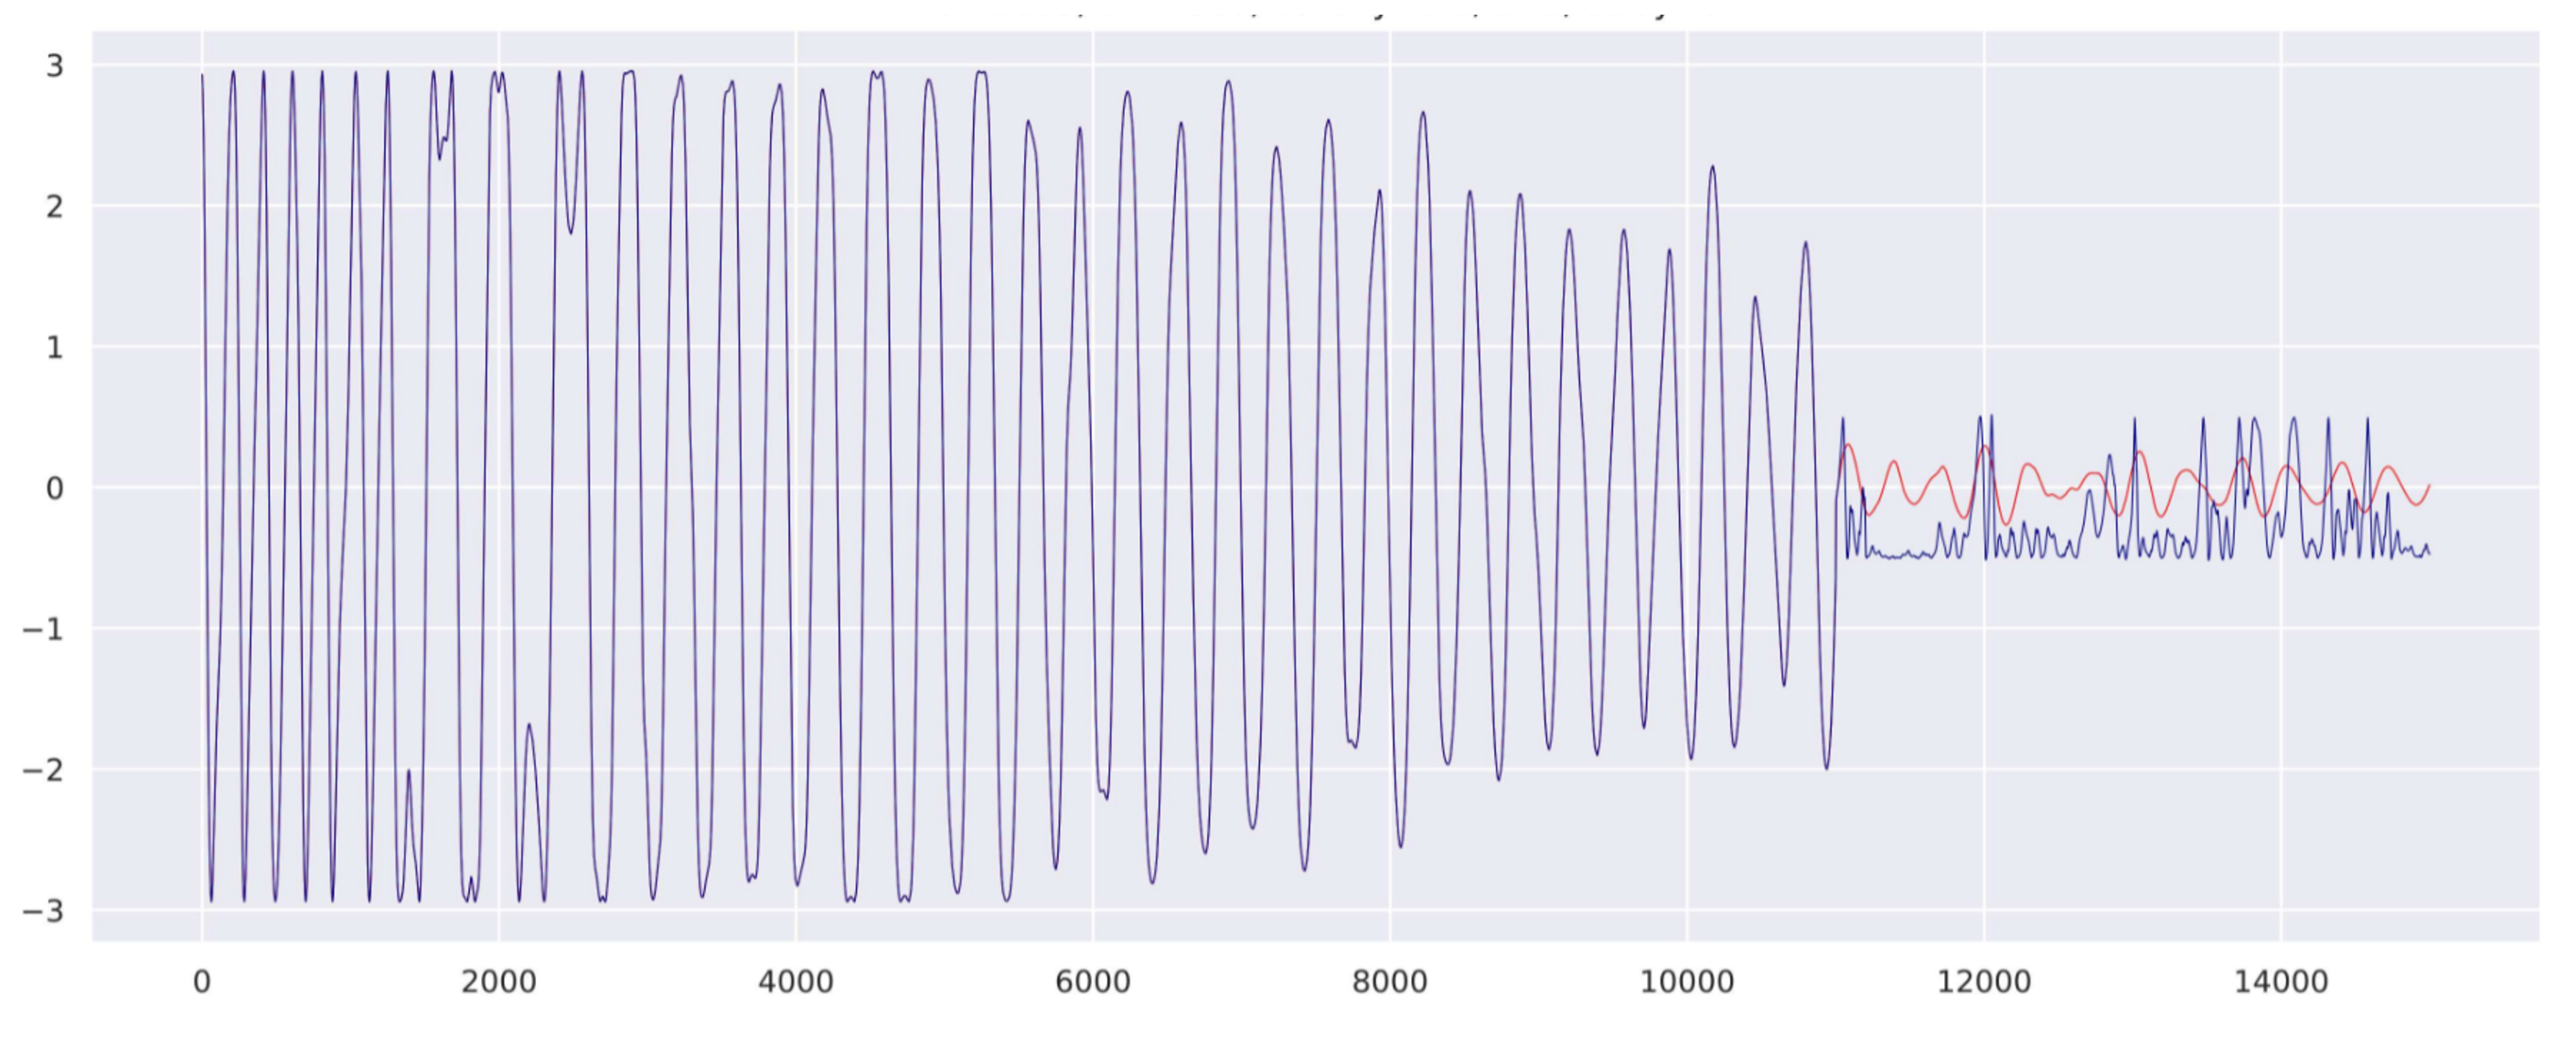
\includegraphics[scale=0.3]{Graphs/_dpfail_nonsurj.eps}
  \centering
\caption{Failure to forecast or learn a map which is not surjective: Evolution of the $y$-coordinate of the bottommost pendulum plotted here for 15000 timestep. Plotted here the predicted value(red) versus the actual value(blue). The plots overlap for the first 10000 steps, the duration of training to learn the map $\Gamma$. Afterwards, the trajectories start diverging and it the predicted value no longer accurately represents the complexity or energy-loss of the actual data. }
\label{fig:dp_notsurjective}
\end{figure}



Having spent ample time to discuss the challenges, we now change tone so as to satisfy the optimist and present a successful run of the DP-data to predict the future movement of the pendulum.

The system was driven for 15500 steps, of which the first 500 were immediately discarded to simulate the network 'forgetting'. The driving function $g$ had input and reservoir matrices were implemented as sparse matrices filled to 20\%. Parameter-values of $\alpha=0.99$ and $a=0.5$ were used.
The remaining 15000 datapoints were used to train a network with 128 neurons. 
The network was initialised to contain 16 hidden layers each with a layer dimension of 64, activated with the tanh activation function.
Training was accomplished using 256 epochs with batch sizes 128 and a delay of 1. See~\ref{fig:dp_success_traj} for results pertaining to the trajectory taken by the DP's components and then~\ref{fig:dp_success_density} to witness associated densities of predicted vs. actual values.


\begin{figure}[ht]
  \centering
  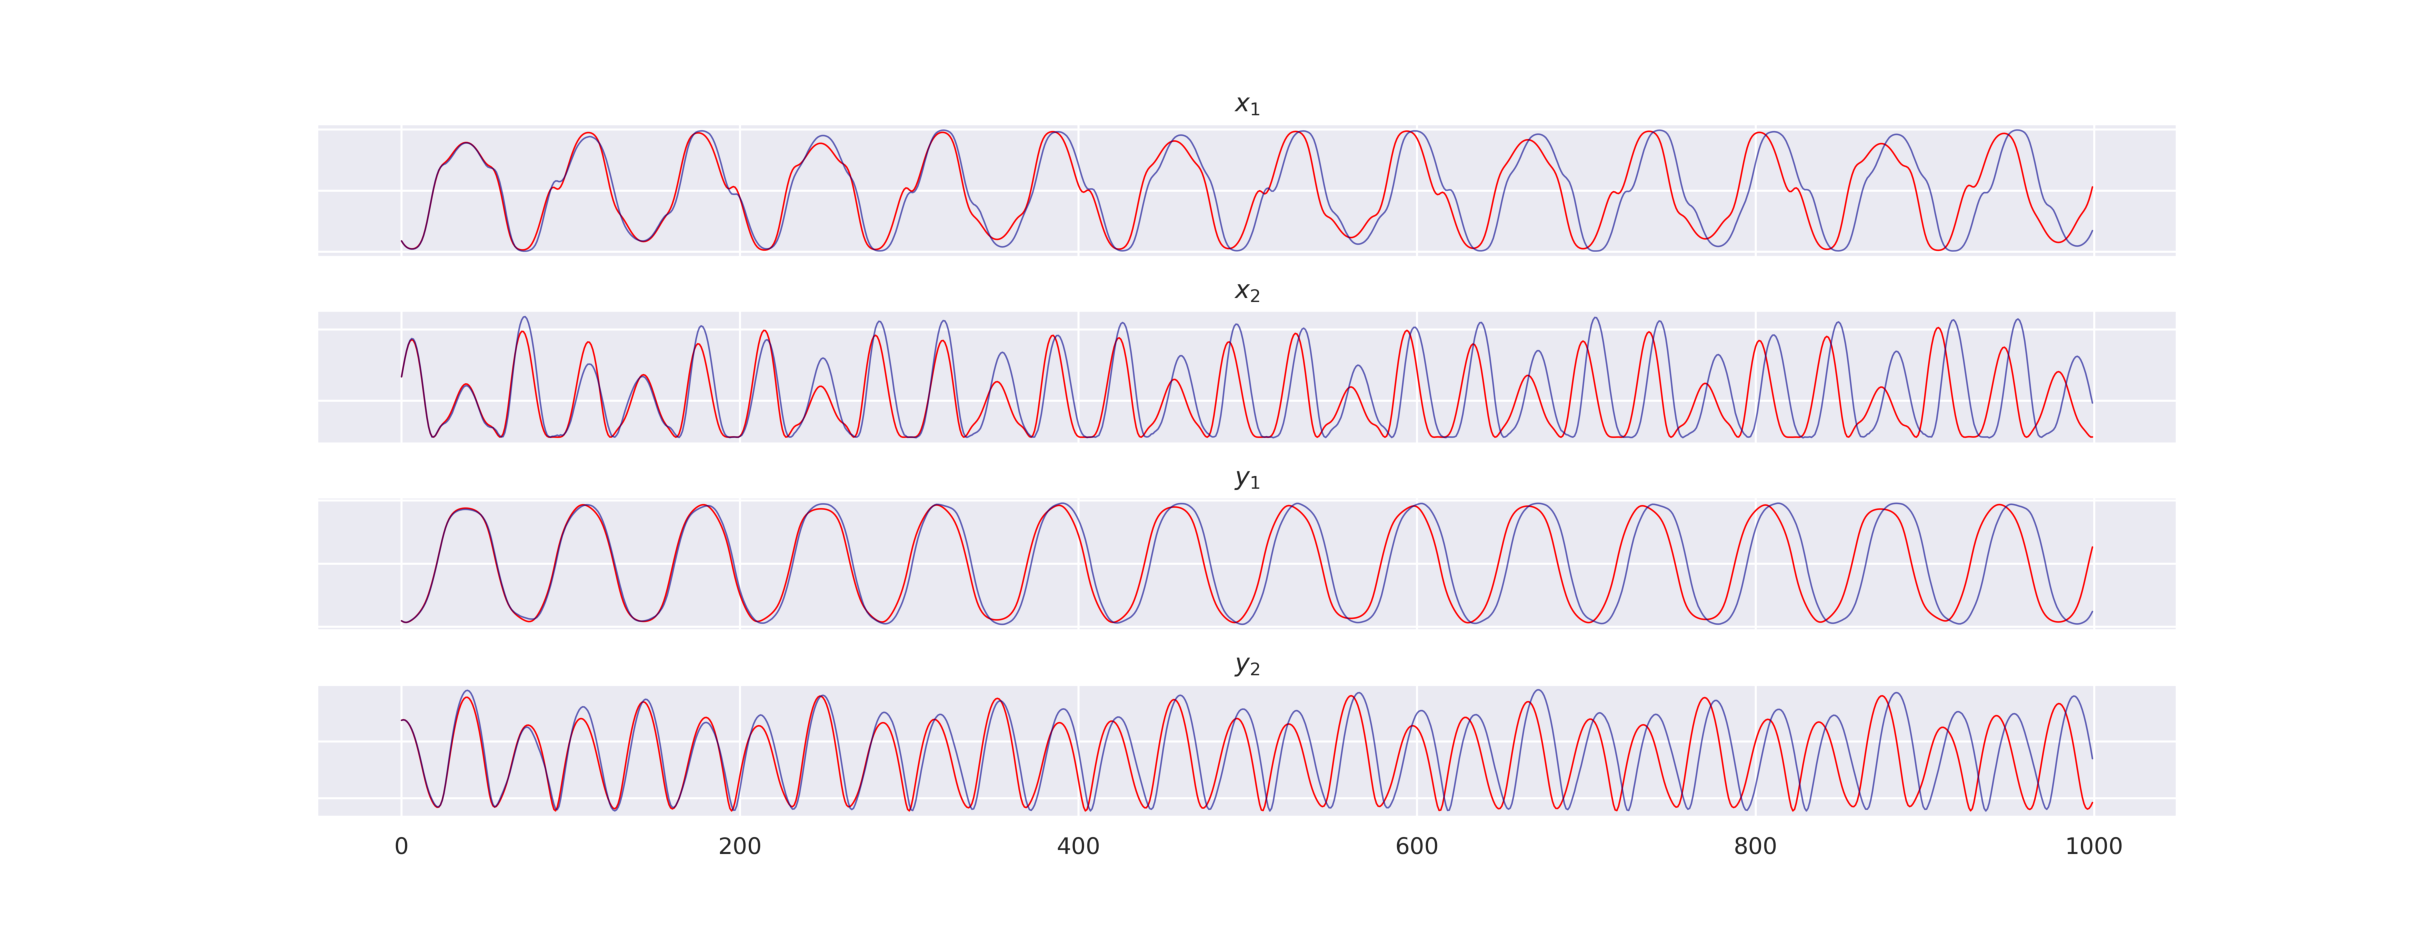
\includegraphics[width=0.95\linewidth]{Graphs/_dp_success_4coords_traj.eps} 
  \captionof{figure}{Predicted(red) and actual(blue) trajectories of the $x$- and $y$-coordinates of each of the pendulum heads. From top to bottom are as follows: $x$-coordinate of topmost pendulum head, $y$-coordinate of topmost pendulum head, $x$-coordinate of lower pendulum head, $y$-coordinate of lower pendulum head. 
  These graphs were constructed by predicting the DP 1000 timesteps into the future and in so doing illustrating the long-term consistency and accuracy of the learnt system. Here we lock onto the near-exact trajectory for about 300 timesteps and stay close up until about 600 seconds.  } 
  \label{fig:dp_success_traj}
\end{figure}
\begin{figure}[ht]
  \centering
  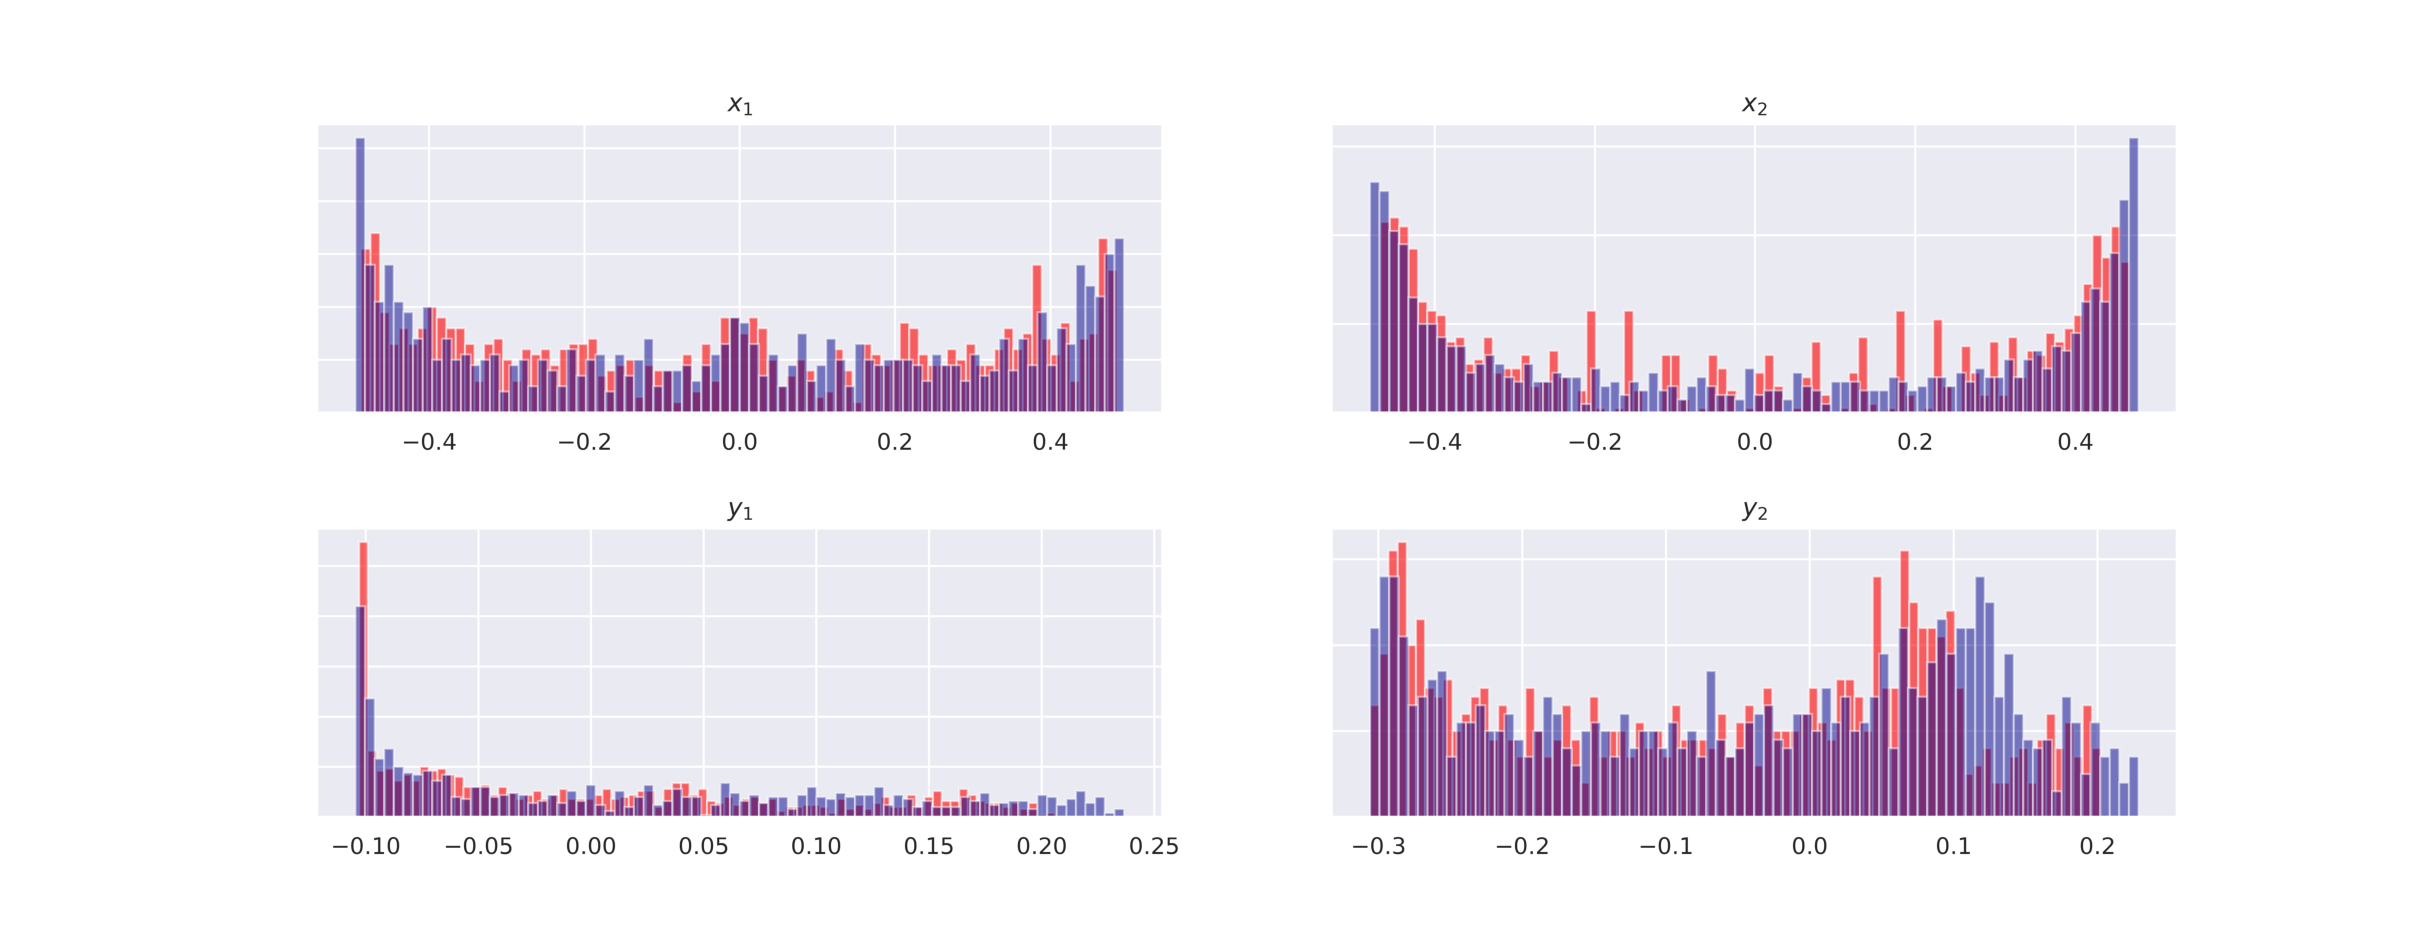
\includegraphics[width=\linewidth]{Graphs/_dp_success_4coords_hist.eps}
  \captionof{figure}{Densities of predicted and actual values of $x$- and $y$-coordinate of pendulum heads.}
  \label{fig:dp_success_density}
 \end{figure}
  

We now consider an experiment where noise is added to the system and find it to be incredibly robust. We employ the same parameters as before and add noise from a normal-distribution with mean zero and standard deviation equal to 0.1 which translates to roughly 39dB's of noise.
(For the signal-to-noise ration we adopt the formula $\text{SNR}_{dB}=10\text{log}_{10}\big(\frac{P_\text{{signal}}}{P_{\text{noise}}}\big)$ where $P_\text{{signal}}$ refers to the variance observed in the normalised data and $P_{\text{noise}}$ represents the variance of the added noise.)

Once again consider the actual and predicted trajectories for the noisy DP dataset in Figure~\ref{fig:noisydp_success_traj}. Next we consider the densities of the predicted and actual values in Figure~\ref{fig:noisydp_success_density} and observe that they display highly similar distributions.

\begin{figure}[ht]
  \centering
  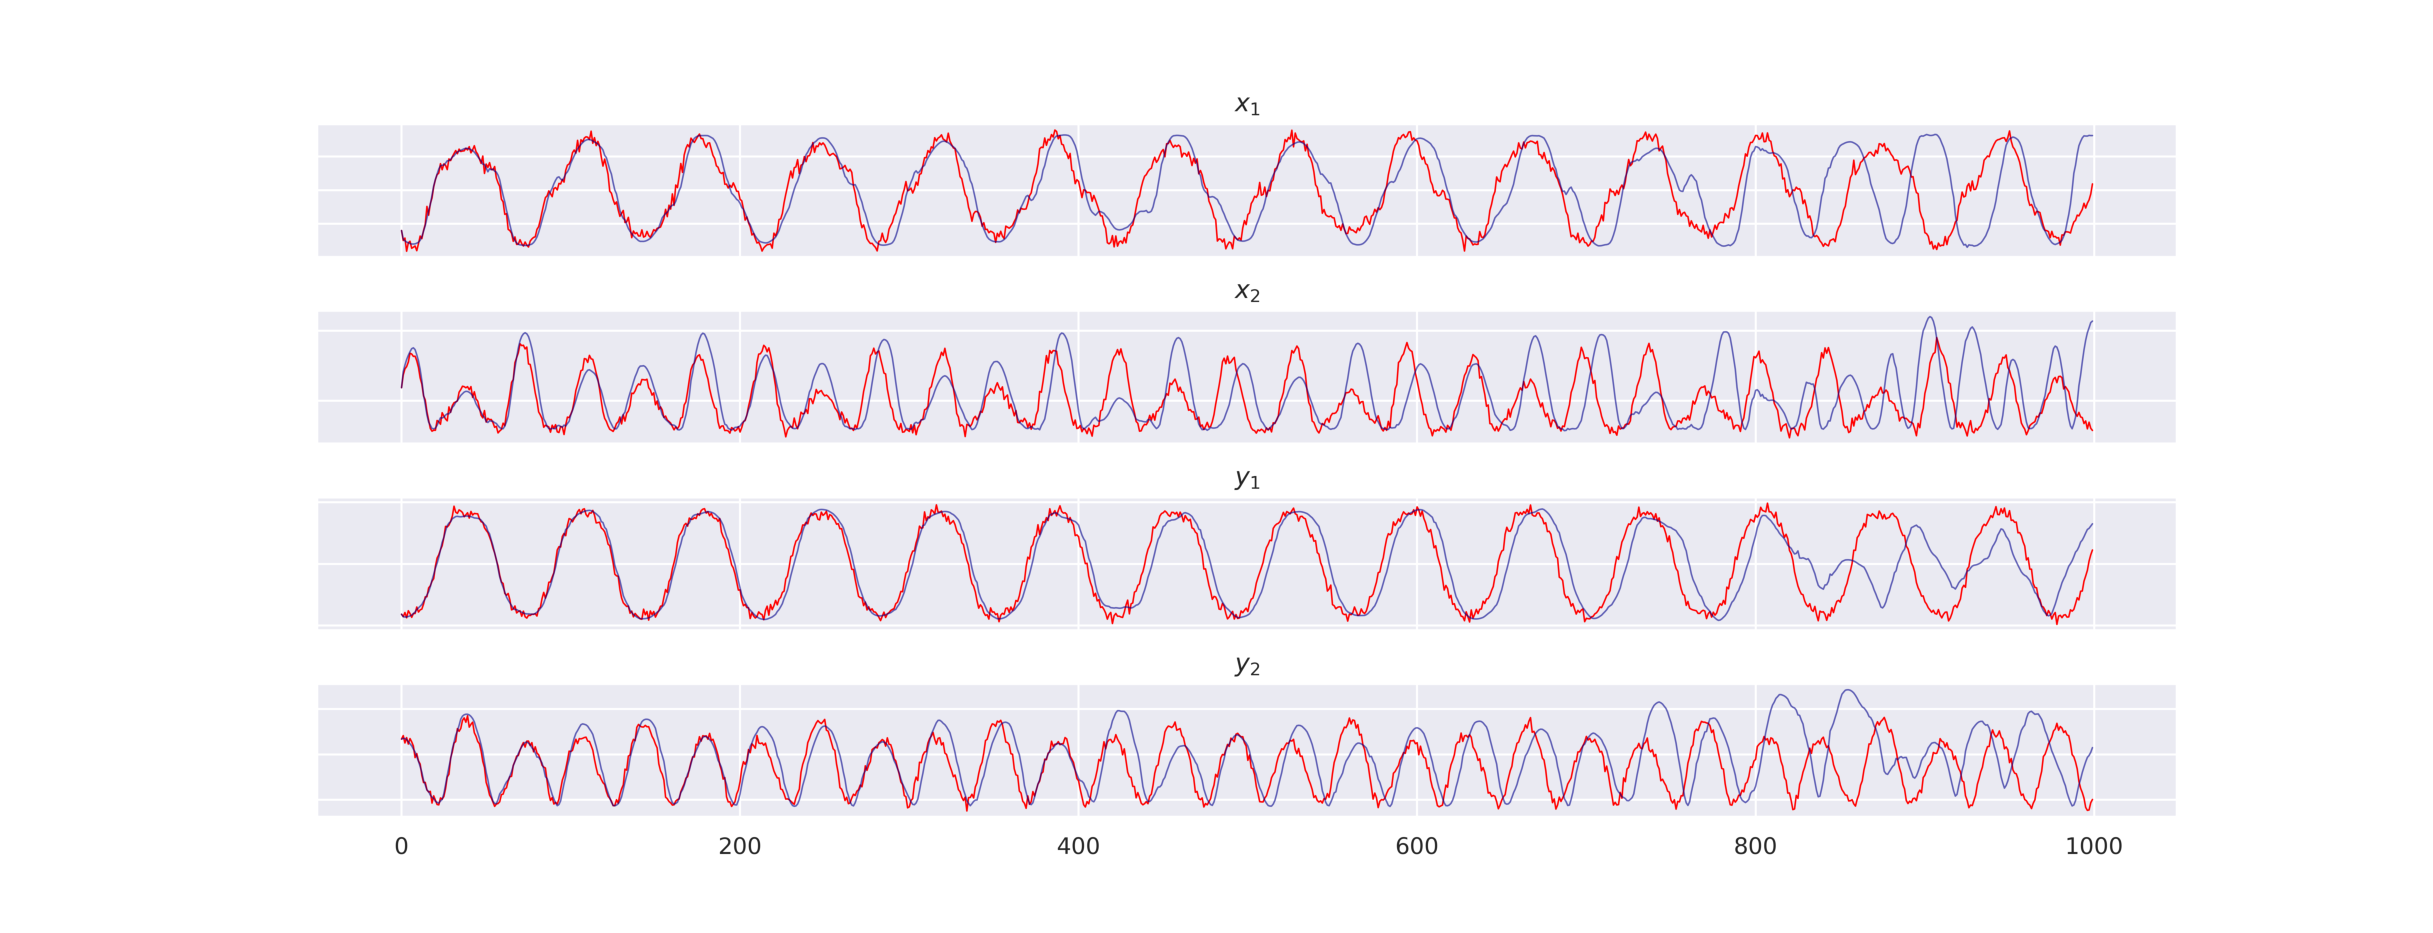
\includegraphics[width=0.95\linewidth]{Graphs/_dp_noise_FigCD_2030.eps} 
  \captionof{figure}{Predicted(red) and actual(blue) trajectories of the $x$- and $y$-coordinates of each of the pendulum heads with noise added from a normal distribution with mean zero and standard deviation 0.1, equating to approximately 39dB's of noise.
  These graphs were constructed by predicting the DP 1000 timesteps into the future and in so doing illustrating the long-term consistency and accuracy of the learnt system. Here we lock onto the near-exact trajectory for about 250 timesteps and stay close up until about 400 seconds.  } 
  \label{fig:noisydp_success_traj}
\end{figure}
\begin{figure}[ht]
  \centering
  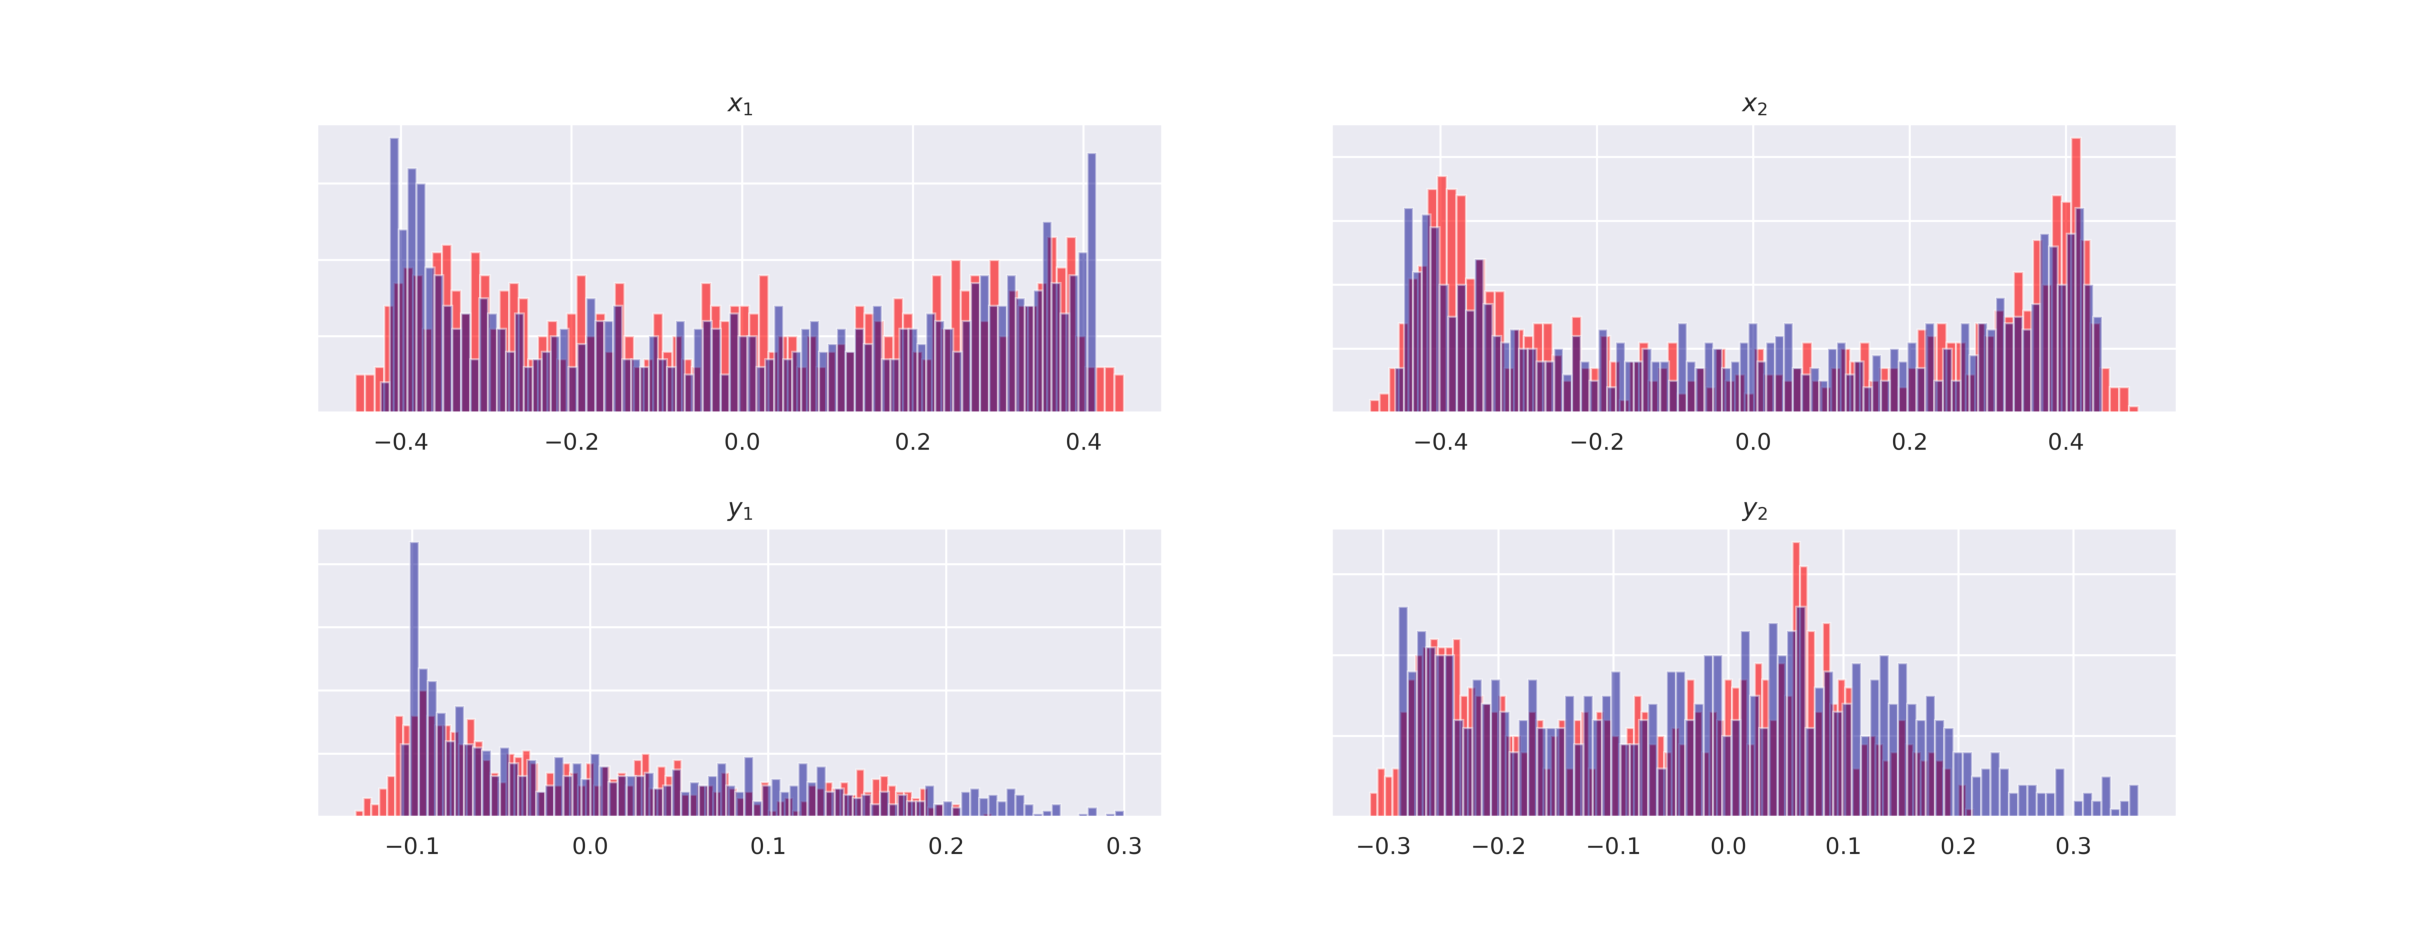
\includegraphics[width=\linewidth]{Graphs/_dp_noise_2B_2030.eps}
  \captionof{figure}{Densities of predicted and actual values of x-coordinate of first pendulum head.}
  \label{fig:noisydp_success_density}
 \end{figure}

 Lastly, a run was done where only a single coordinate (the $y$-coordinate of the lower pendulum head) was fed into the system and we can illustrate through the obtained success that the coordinate contains all the information in its past states necessary to forecast its future evolution.
 \textbf{Insert graphs here. Had to quickly change something here.}
 

\subsection{Additional Attractors: Clifford \& Thomas}
We follow the methodology presented in \cite{manjunath2021universal} but opt to consider attractors different from the Lorenz system and H\'enon map in this project.

\subsubsection{Thomas' Cyclically Symmetric Strange Attractor}\label{Thomas_Attractor}
Thomas' Cyclically Symmetric Strange Attractor, a 3D attractor proposed in 1999 by Ren\'e Thomas in \cite{ThomasAttractor}, is described by a set of three equations which is distinctly reminiscent of the Lorenz system, another deterministic three-equation model exhibiting chaotic behaviour.It has a single parameter $\beta$ and has been shown to transition to chaotic behavious when $\beta<0.208186$~\cite{Thomas_BetaParameter}.
\begin{eqnarray}\label{eqns_thomas}
  x_{n+1} = \sin(y_n) - \beta{x_n} \\
  y_{n+1} = \sin(z_n) - \beta{y_n} \\
  z_{n+1} = \sin(x_n) - \beta{z_n}
\end{eqnarray}

The behaviour of the system with a $\beta$-parameter value of 0.1056 was simulated by scaling it to fit inside the interval $[-1,1]$. Two cases were considered: noise-free and the one perturbed by noise. Noise was generated from a normal distribution with mean 0 and standard deviation 0.05, which to translates approximately 33dB. 
($\text{SNR}_dB$ is calculated exactly as for the DP-data above)

A sequence of 3000 observations in both the clear and noisy data-sets respectively were fed into the system with 300 entries discarded to simulate the network's loss of memory. The next 9000 steps were predicted and compared with true data.

\begin{figure}[ht]
  \centering
  \minipage{0.5\linewidth}
    \centering
    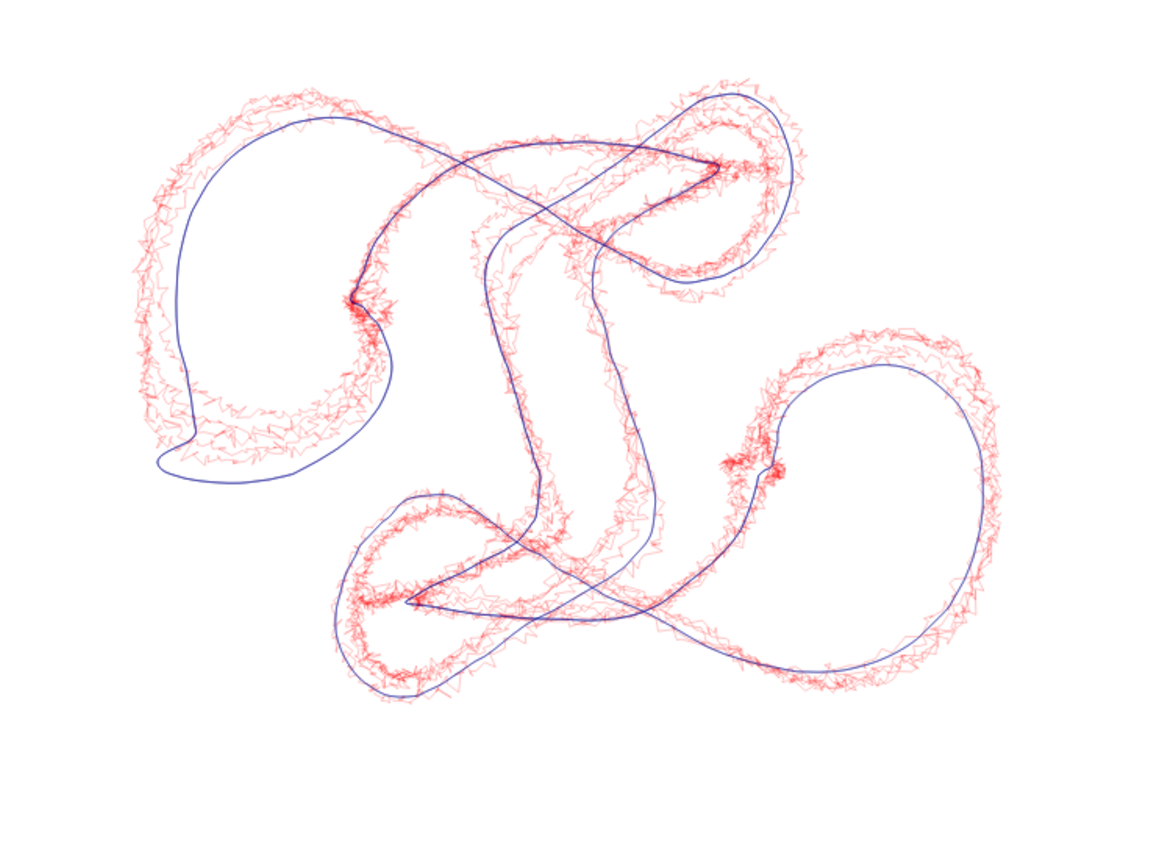
\includegraphics[width=0.8\linewidth]{Graphs/_thomas_noisy_0.1056.eps}
  \endminipage\hfill
  \minipage{0.5\linewidth}
    \centering    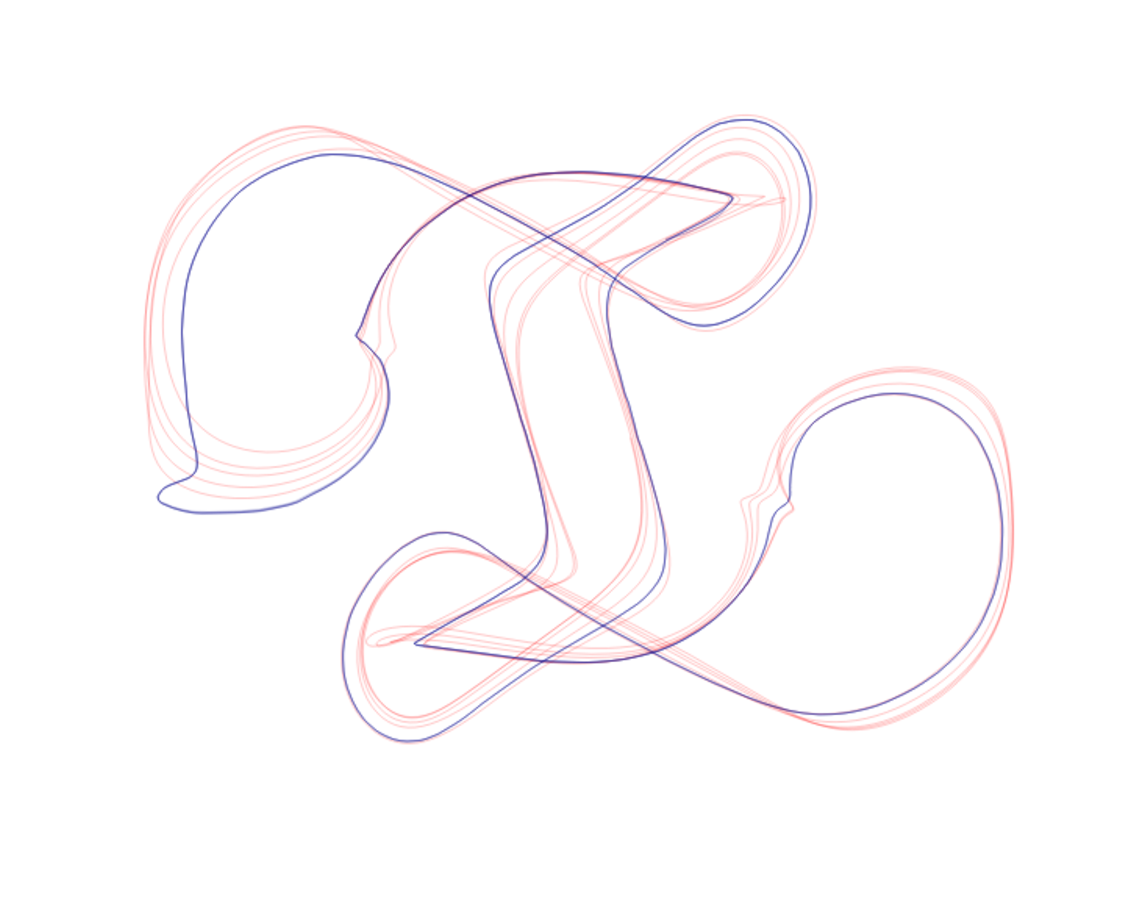
\includegraphics[width=0.8\linewidth]{Graphs/_thomas_clean_0.1056.eps}
  \endminipage
  \captionof{figure}{True(red) and predicted(blue) trajectories for the Thomas attractor with parameter value $\beta=0.1056$. To the left: Noise added from normal distribution with mean zero and standard deviation 0.05. Right: No noise added to dataset.}
\end{figure}


The RNN was initialised as follows: the dimension of the network is set equal to 500 neurons and 12 hidden layers of dimension 64 each were initialised. Training is realised through 150 epochs of batch sizes of 128 each; the map is learnt via the Adam Optimiser using finer and finer learning rates (0.001 and then divided by 10 at every iteration).

\begin{figure}[ht]
  \centering
  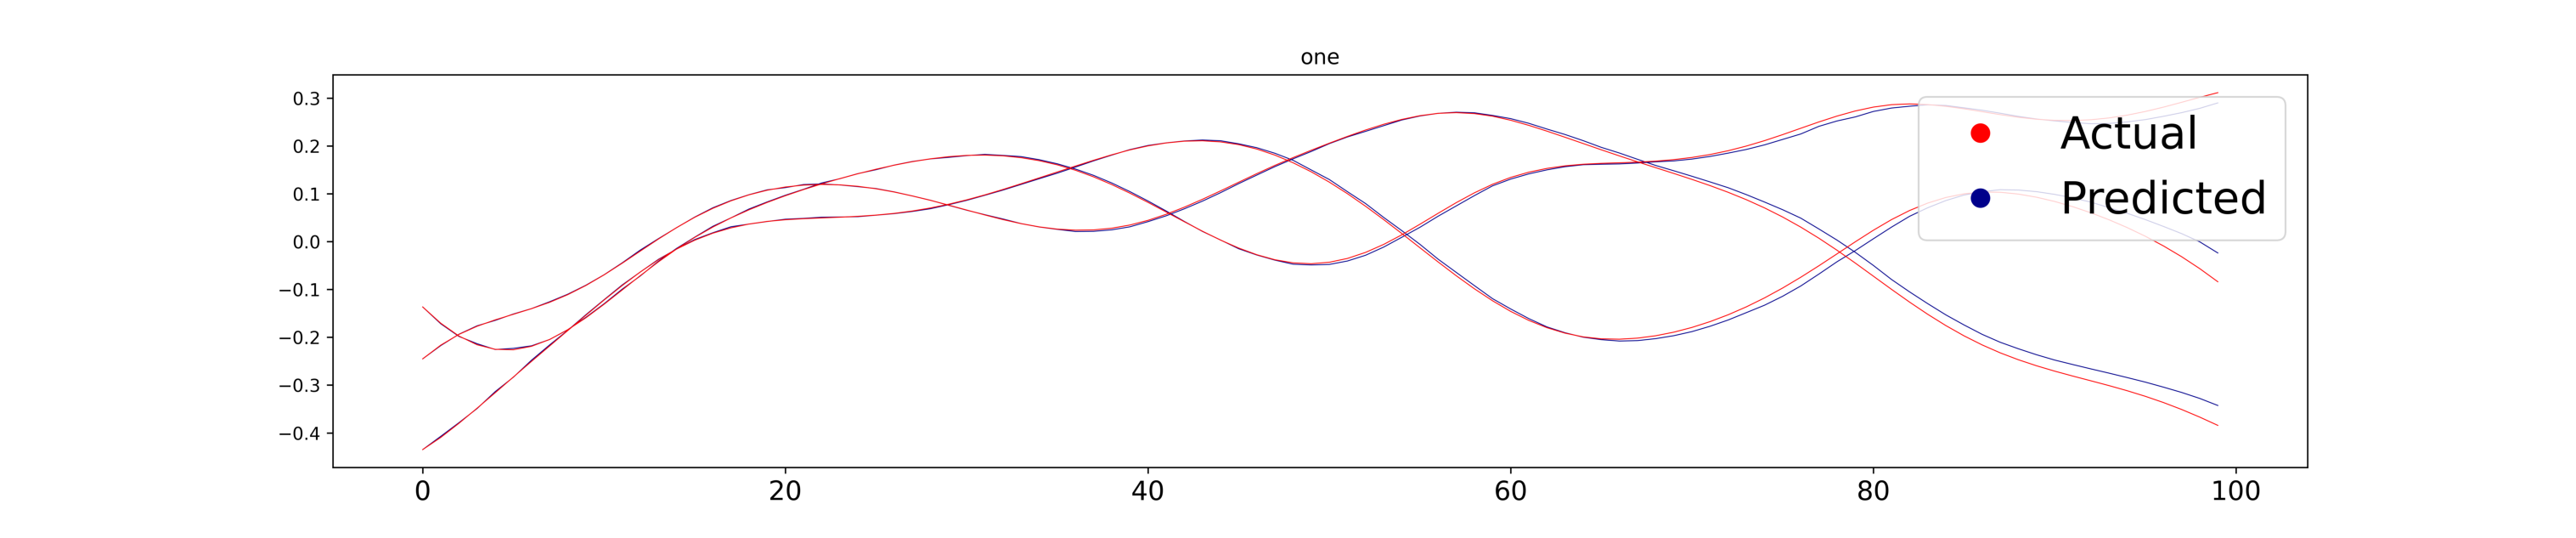
\includegraphics[scale=0.35]{Graphs/_Thomas_1.eps}\caption*{Predicted trajectories of the $x$- and $y$-coordinates for the Thomas attractor with parameter-value $\beta=0.1056$ demonstrate empirically the ability to predict the evolution of the trajectory for the next an estimated 100 timesteps into the future near-exactly. Here no noise was added.}
  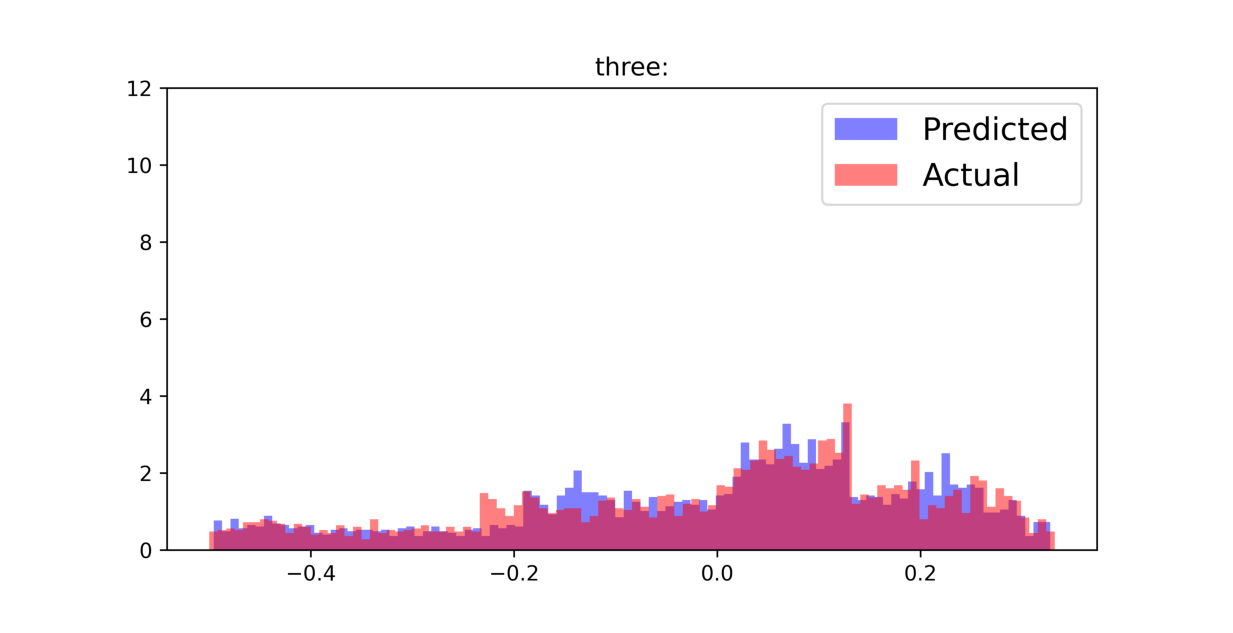
\includegraphics[scale=0.5]{Graphs/_Thomas_3.eps}\caption*{Represented here the learnt (blue) and actual (red) densities of the first coordinate ($x$-coordinate) of the dataset for the Cyclically Symmetric Attractor with parameter-value $\beta=0.1056$.}
\end{figure}


\subsubsection{Fractal Dream Attractor}

Another 2-equation discrete-time map named the Fractal Dream Attractor, or more commonly known as the Pickover Map (first discovered by Clifford A. Pickover and discussed in his fascinating book "Chaos in Wonderland"\cite{PickoverChaos}), was also considered.
\begin{eqnarray}\label{eqns_clifford}
  {x_{n+1}=\sin(ay_n) + c\cos(ax_n)} \\
  {y_{n+1}=\sin(bx_n)+d\cos(by_n)}
\end{eqnarray}

\begin{figure}[ht]
  \centering
  
\includegraphics[width=1.0\textwidth,left]{Graphs/_Clifford_1_nonoise.eps}
  \caption*{These graphs were constructed by predicting the Clifford system 1000 steps into the future and in so doing illustrating the long-term consistency and accuracy of the learnt system. As perceived here, we are able to lock on to the trajectory of the Clifford map almost exactly for the first 25 steps.}
  \minipage{0.5\textwidth}
      \centering
      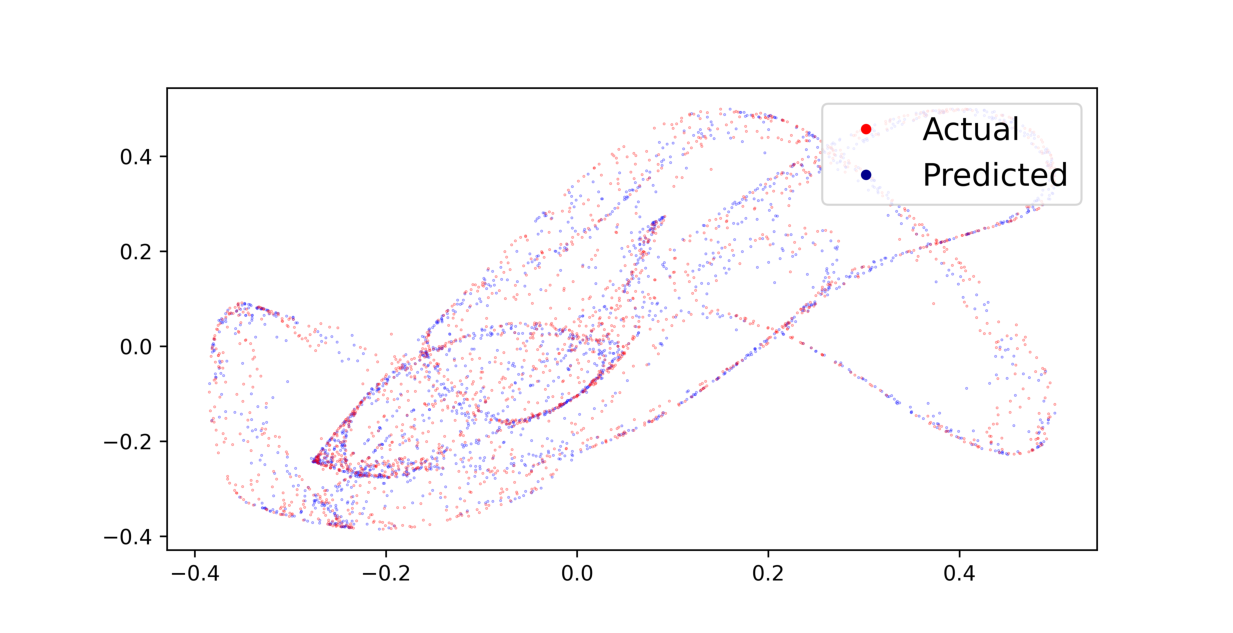
\includegraphics[width=\linewidth]{Graphs/_Clifford_2_nonoise.eps}
  \endminipage\hfill
  \minipage{0.5\textwidth}
    \centering
    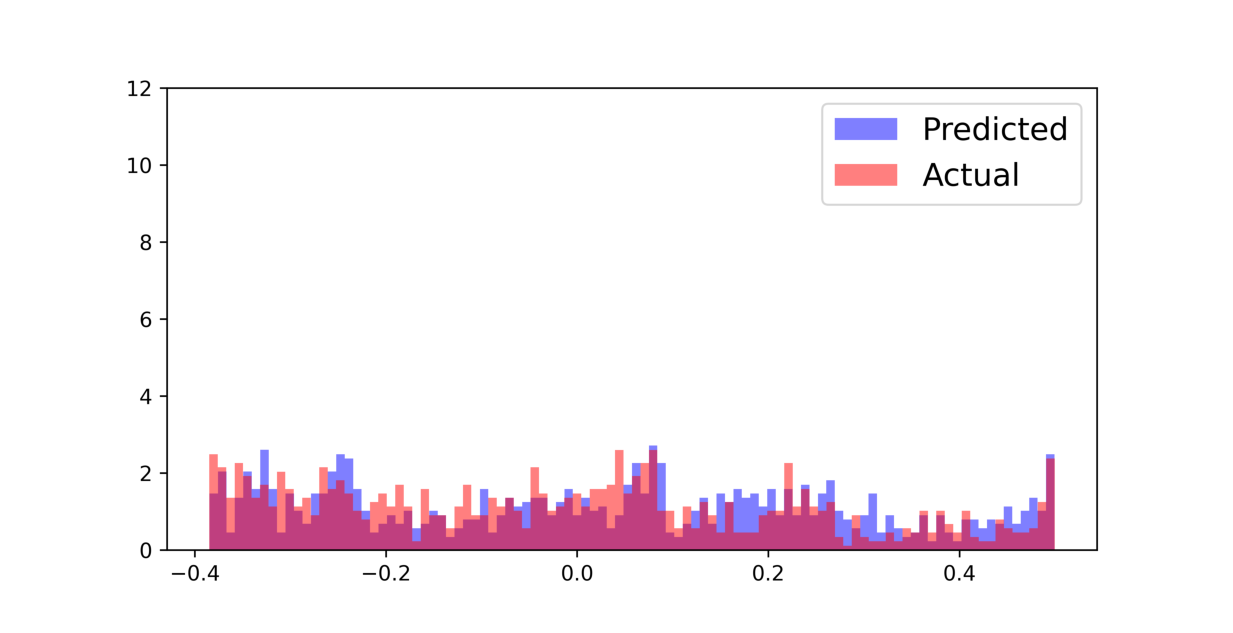
\includegraphics[width=\linewidth]{Graphs/_Clifford_3_nonoise.eps}
  \endminipage
  \caption{The bottom row, left, shows a plot of the true attractor(red) and the predicted values(blue). Bottom row, right, shows the distribution of the first coordinate of the learnt system (blue) and the actual Clifford system (red). }
  \label{fig:Clifford}
\end{figure}

The behaviour of the system with a parameter values of $x_0=0$, $y_0=0$, $a = -1.7$,  $b = 1.8$, $c = -1.9$ and $d = -0.4$ was examined.
Data was scaled to fit inside the interval $[-1,1]$. Only the noise-free case was investigated. 
 A sequence of 25000 observationswas fed into the system with 15000 entries discarded to simulate the network's loss of memory. The next 1000 steps were predicted and compared with true data.
The RNN was initialised exactly as for Thomas' Cyclically Symmetric Strange attractor: the dimension of the network is set equal to 500 neurons and 12 hidden layers of dimension 64 each were initialised. Training is realised through 150 epochs of batch sizes of 128 each; the map is learnt via the Adam Optimiser using finer and finer learning rates (0.001 and then divided by 10 at every iteration).

\section{Functional Complexity Reduction in Noninvertible maps}

% Besides being able to learn the action of the Koopman operator exactly, our setup has other advantages over selecting or optimizing the choice of observables as in the Extended Dynamic Mode Decomposition (EDMD) algorithm (see, [21, 22]). We can alter the functional complexity of G T by changing the number of observables or equivalently by altering the dimension of X – in the case of a RNN implementation of g, by simply changing the number of neurons in the network. Empirically, increasing the dimension of X is found to increase the linear relationship (or intuitively reduces the functional complexity of G T ) that is measured as a generalization of the Pearson correlation coefficient to random vectors (see, [44]) between (x_{n−1} , x_{n}) and G_T (x_{n−1} , x_n), and such numerical evidence is tabulated in [11, Table 1]. In contrast, expanding the set of observables while using EDMD to learn a map with a lower functional complexity is a highly involved task, not least because so much that one often does not know how to guess a new observable, as well as the fact that adding observables does not necessarily retain the invariance of the span of the observables.

% Empirical evidence shows that a linearity measure like a Pearson correlation coefficient points at reduced functional complexity while learning the dynamics in the state space of the driven system.

% Empirically (see Table ??), increasing the dimension of X is found to increase the linear relationship
% (or intuitively reduce the functional complexity of G T ) that is measured as a generalization of the Pearson correlation coefficient to random vectors (see, [?]) between (x n−1 , x n ) and G T (x n−1 , x n ). If Σ a and Σ b denotes the covariance matrices of the vectors (x n−1 , x n ) and G T (x n-1 , x n ) respectively, and if Σ ab denotes the covariance matrix between the vectors (x n-1 , x_n ) and G_T (x n-1 , x_n ), then the multidimensional 18correlation coefficient is computed by using the traces of these matrices: 
% \[\pho = \frac{tr(\sum_{ab})}{tr(\sqrt{\sum_{a}\sum_{b}})}\]

% This multidimensional correlation coefficient satisfies most of the well-known properties of the one-dimensional Pearson coefficient. In particular, ρ = ±1 if and only Y = AX + b for some invertible matrix A and vector b. Hence ρ, and in practice, the estimator ρ̂, can be used to measure the linear relationship between two random vectors of the same dimension and thus serves as an indicator of functional complexity.

% We remark that the estimation of such linear relationship in (see Table ??) obtained by sample correlations alone is justified whenever {u n } is a realization of an ergodic process since then when g has the USP, any solution {x n } is also a realization of an ergodic process [?]. In the ergodic input case the generalized Pearson correlation coefficient (between (x n−1 , x n ) and G T (x n−1 , x n )) is independent of n.



In the case of non-invertible maps, we note that the map $G_T$ is a homemorphism although $T$ is not. Further, empirically it is found that $G_T$ is much more linear than $T$ as measured by what is called the multidimensional correlation coefficient $\rho$. This coefficient is a generalization of the Pearson correlation coefficient for real-valued random variables to random vectors (see, \cite{puccetti2019measuring}). We state teh details of computing this coefficient between 
$(x_{n-1},x_n)$ and $G_T(x_{n-1},x_n)$. 
If $\Sigma_{a}$ and $\Sigma_{b}$ denotes the covariance matrices of the vectors $(x_{n-1},x_n)$ and $G_T(x_{n-1},x_n)$ respectively, and if $\Sigma_{ab}$ denotes the covariance matrix between the vectors $(x_{n-1},x_n)$ and $G_T(x_{n-1},x_n)$, then the multidimensional correlation coefficient is computed by using the traces of these matrices:
\[
    \rho= \frac{\text{tr}({\Sigma_{ab}})}{\text{tr}({\sqrt{\Sigma_a\Sigma_b}})}.
\]
This multidimensional correlation coefficient satisfies one of the desired and well-known properties of the one-dimensional Pearson coefficient. That is, $\rho=\pm 1$ if and only if $Y\overset{d}{=}AX+b$ for some invertible matrix $A$ and vector $b$. Hence $\rho$, and in practice can be used  to measure the linear relationship between two random vectors of the same dimension and thus serves as an indicator of functional complexity. For the non-invertible system defined by the Clifford attractor, we indicate the difference by which $\rho$ changes for $G_T$ in Table~\ref{tbl_attractorsPearson}.
Following \cite{manjunath2021universal}, we say that this multidimensional correlation coefficients $\rho$ to evidence a general reduction in the functional complexity of the map $G_T$ emerging due to a RNN. In the 
Table ~\ref{tbl_attractorsPearson}, the second column corresponds to the amount of artificial neurons (the dimension of $X$) in the implemented RNN.
               
  
\begin{center}
  \begin{table} 
      \scalebox{0.75}
      {\begin{tabular}{|c|c| c c |} 
          \hline
          Input & Dimension of $X$ & $u_n$ vs $u_{n+1}$ 
          & $\begin{bmatrix}
              x_{n-1}\\
              x_n
          \end{bmatrix}$ vs $\begin{bmatrix}
              x_n\\
              x_{n+1}
          \end{bmatrix}$ \\
          \hline      
          % \hline
          % $(w_n)$ is the Lorenz states, sampled every 0.1 timestamps. & & &\\
          % \multirow{3}{*}{$u_n=\frac{1}{100}w_n$} & 10 &0.9311  & 0.9731\\
          %     & 100 &  & 0.9934\\
          %     & 1000 & & 0.9930\\              
          % \multirow{3}{*}{$u_n=\frac{1}{10}(\sin(0.1w_{n,x})+\sin(0.1w_{n,y})+\sin(0.1w_{n,z}))$} 
          %     & 10 &0.8401  & 0.9392\\
          %     & 100 & & 0.9616\\
          %     & 1000 & & 0.9737\\
          % \hline         
          
          
               \hline  
               $(w_n)$ comes from the Clifford Attractor \\ (for $a = -1.7; b = 1.8; c = -1.9; d = -0.4$): & & & \\
        {$w_{n+1}= \begin{bmatrix} \sin(aw_{n,y}) + c\cos(aw_{n,x}) \\ 
                                                                    \sin(bw_{n,x})+d\cos(bw_{n,y}) \end{bmatrix}$} & & & \\
          \multirow{3}{*}{$u_n = w_n-\overline{w}$}
              & 10 & -0.21713 & 0.78719 \\
              & 100 & &  0.8334 \\
              & 1000 & & 0.84854 \\
          % \hline 
          % $(w_n)$ comes from the Logistic map: & & & \\
          % {$ w_{n+1}  = 4w_n(1-w_n)$} & & & \\
          % \multirow{3}{*}{$u_n = w_n - 0.5$} 
          %     & 10 &-0.0314  & 0.5577\\
          %     & 100 &  & 0.7150\\
          %     & 1000 & & 0.7826\\
          % \hline
          % \hline
          % $(w_n)$ comes from the Svensson Attractor \\ (for $a = -1.7; b = 1.8; c = -1.9; d = -0.4$): & & & \\
          % {$w_{n+1}= \begin{bmatrix} d\sin(aw_{n,x}) - \sin(bw_{n,y}) \\ 
          %                                                             c\cos(aw_{n,x})+\cos(bw_{n,y}) \end{bmatrix}$} & & & \\
          %   \multirow{3}{*}{$u_n = w_n-\overline{w}$}
          %       & 10 & -0.2243 & 0.49698 \\
          %       & 100 & &  0.63310 \\
          %       & 1000 & & 0.71151 \\
           \hline
                \end{tabular}} %\ednote{http://paulbourke.net/fractals/peterdejong/}
 \label{Table_FC}
 \caption{Following \cite{manjunath2021universal}, we determine the multidimensional correlation coefficients $\rho$ to evidence a general reduction in the functional complexity of the map $G_T$ emerging due to a RNN. Rows correspond to distinct dynamical systems considered in the experiments
      The second column corresponds to the amount of artificial neurons (the dimension of $X$) in the implemented RNN.
      The last two columns comprise numerical estimates of $\rho$ for the relevant vectors. The linear association between $u_n$ vs $T(u_{n})$, as well as the linear relationship $\begin{bmatrix}
              x_{n-1}\\
              x_n
          \end{bmatrix}$ vs $G_T \left( \begin{bmatrix}
              x_{n-1}\\
              x_n
          \end{bmatrix}\right)$ may be contrasted by the reader. 
          Finally, the RNN's dimension (from \eqref{Seq_RNN}) is provided to exhibiting that an increase in dimension of the driven system will 
          typically result in a map $G_T$ with less functional complexity.}.
      \end{table}\label{tbl_attractorsPearson}
\end{center}

  